\documentclass[11pt,a4paper]{article}

\usepackage[margin=1in,headheight=22pt]{geometry}
\usepackage{amsmath,amssymb}
\usepackage{booktabs}
\usepackage{microtype}
\usepackage{xcolor}
\usepackage{tikz}
\usetikzlibrary{arrows.meta,positioning}
\usepackage{pgfplots}
\pgfplotsset{compat=1.18}
\usepackage{float}
\usepackage{caption}
\usepackage{subcaption}
\usepackage{titlesec}
\usepackage{fancyhdr}

\definecolor{ink}{HTML}{1C2833}
\definecolor{real}{HTML}{1F4E79}
\definecolor{rand}{HTML}{B03A2E}
\definecolor{plain}{HTML}{1A7A6D}
\definecolor{muted}{HTML}{7B8794}
\definecolor{rule}{HTML}{D5D0C8}
\definecolor{paper}{HTML}{F7F5F0}

\titleformat{\section}{\large\bfseries\color{ink}}{\thesection}{0.7em}{}[\vspace{0.25em}{\color{rule}\titlerule}]
\titleformat{\subsection}{\normalsize\bfseries\color{ink}}{\thesubsection}{0.6em}{}
\titlespacing*{\section}{0pt}{1.25em}{0.65em}
\titlespacing*{\subsection}{0pt}{1.0em}{0.35em}

\pagestyle{fancy}
\fancyhf{}
\fancyhead[L]{\small\color{muted}{Entropy of hidden maps}}
\fancyhead[R]{\small\color{muted}{\thepage}}
\renewcommand{\headrulewidth}{0.4pt}
\renewcommand{\headrule}{\hbox to\headwidth{\color{rule}\leaders\hrule height \headrulewidth\hfill}}
\fancypagestyle{plain}{\fancyhf{}\renewcommand{\headrulewidth}{0pt}}

\captionsetup{font=small, labelfont=bf, skip=0.55em}
\pgfplotsset{
  every axis/.append style={
    label style={font=\small,color=ink},
    tick label style={font=\footnotesize,color=ink},
    legend style={font=\footnotesize, fill=white, fill opacity=0.94, text opacity=1, draw=rule, inner sep=3pt},
    axis line style={ink},
    tick style={ink},
    scale only axis,
    line width=1.05pt
  }
}

\begin{document}

\begin{center}
{\LARGE\bfseries Entropy of hidden maps in a network}\\[0.55em]
{\large 9 October 2026}
\end{center}
\vspace{0.4em}

\section{The question}

A network does not only store a final answer. At each layer it builds a hidden map of the picture it was shown. That map can be simple, with its energy gathered in a few spatial frequencies, or busy, with its energy spread over many frequencies.

The question is whether this spread behaves differently in two situations. In the first, the network is learning the real labels of the pictures. In the second, the labels have been shuffled, so the network can only memorize an arbitrary assignment.

\section{The number on the graphs}

The number plotted below is called hydrodynamic entropy. It was defined for fluid flows, and the same arithmetic applies to any two-dimensional field, including a hidden map.

Take one map. Subtract its average value, so a flat offset does not count as structure. Apply a smooth window at the edges, because the map is not a repeating pattern. Transform it into spatial frequencies, and measure the energy at each frequency. Turn those energies into shares that add up to one. The entropy is high when the shares are even, and low when a few frequencies hold almost everything. Dividing by the largest possible value puts every map on the same scale, from 0 to 1.
\begin{equation}
  \widetilde S
  = \frac{1}{\log_2 M}
    \left(-\sum_{\mathbf{k}} p_{\mathbf{k}}\log_2 p_{\mathbf{k}}\right),
  \qquad
  p_{\mathbf{k}} = \frac{E(\mathbf{k})}{\sum E},
  \qquad
  M = H \times W.
\end{equation}
A constant field scores 0. A field of random noise scores close to 1. The graphs use the last map in the network, which is \(8\times 8\), unless a figure says otherwise.

\begin{figure}[H]
\centering
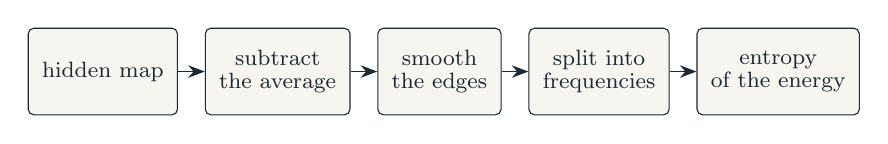
\begin{tikzpicture}[
  font=\footnotesize,
  box/.style={draw=ink, rounded corners=2pt, align=center, inner sep=5pt, fill=paper, text=ink, minimum height=11mm},
  arr/.style={-{Stealth[length=2.1mm]}, semithick, ink}
]
  \node[box] (field) {hidden map};
  \node[box, right=3.4mm of field] (prep) {subtract\\[-0.15em]the average};
  \node[box, right=3.4mm of prep] (win) {smooth\\[-0.15em]the edges};
  \node[box, right=3.4mm of win] (fft) {split into\\[-0.15em]frequencies};
  \node[box, right=3.4mm of fft] (ent) {entropy\\[-0.15em]of the energy};
  \draw[arr] (field) -- (prep);
  \draw[arr] (prep) -- (win);
  \draw[arr] (win) -- (fft);
  \draw[arr] (fft) -- (ent);
\end{tikzpicture}
\caption{From one hidden map to the number on the vertical axis.}
\label{fig:pipeline}
\end{figure}

\clearpage
\section{The result}

\begin{figure}[H]
\centering
\begin{tikzpicture}
\begin{axis}[
  xlabel={epoch},
  ylabel={entropy of the last map},
  xmin=-1, xmax=40,
  ymin=0.68, ymax=0.93,
  width=0.86\textwidth,
  height=6.3cm,
  legend to name=condlegend,
  legend columns=2,
  legend cell align={left},
]
\addplot[real, mark=*, mark size=1.15pt] table[x=epoch, y=s_late] {figures/real_reg.dat};
\addlegendentry{real labels, with augmentation}
\addplot[rand, mark=*, mark size=1.15pt] table[x=epoch, y=s_late] {figures/random_plain.dat};
\addlegendentry{shuffled labels, no augmentation}
\addplot[plain, dashed] table[x=epoch, y=s_late] {figures/real_plain.dat};
\addlegendentry{real labels, no augmentation}
\addplot[muted, dashed] table[x=epoch, y=s_late] {figures/random_reg.dat};
\addlegendentry{shuffled labels, with augmentation}
\end{axis}
\end{tikzpicture}
\par\vspace{0.45em}
\pgfplotslegendfromname{condlegend}
\caption{Entropy of the \(8\times 8\) map while the network trains on \(10{,}000\) pictures.
Epoch \(-1\) is the network before any training.
The vertical axis is a window inside the full range, which runs from 0 to 1.
Each line is a mean over seeds. Seeds differ by less than \(0.01\) at the end.}
\label{fig:entropy}
\end{figure}

Figure~\ref{fig:entropy} is the main result. Before training, every run starts near \(0.83\): a random network already spreads energy fairly widely. The first epoch pulls the entropy down, to about \(0.71\) for real labels and about \(0.73\) for shuffled labels. After that, the lines separate.

With real labels, and with the usual cropping, flipping, and penalty on large weights, the entropy stays low. It ends at \(0.76\). Test accuracy on the real labels ends at \(0.81\).

With shuffled labels, and with that cropping and penalty turned off, the entropy turns around and climbs. It is back near its starting value by epoch 20, and it finishes at \(0.90\). Accuracy on the real test labels stays at \(0.10\), which is the score of guessing among ten classes. The climb is already clear when accuracy on the shuffled training labels is still only about \(0.15\). Fitting the shuffle has barely started, and the last map is already becoming more spread out.

The two dashed lines are the checks. Real labels with cropping and the weight penalty removed still end at \(0.79\), even though the network has learned the training set perfectly. Shuffled labels with cropping and the penalty left on also end at \(0.79\), and that network never really fits. The rise in Figure~\ref{fig:entropy} needs both ingredients: a shuffled target, and freedom to fit it. Either one alone leaves the entropy with the real-label lines.

\begin{figure}[H]
\centering
\begin{subfigure}[t]{0.48\textwidth}
\centering
\begin{tikzpicture}
\begin{axis}[
  xlabel={epoch},
  ylabel={accuracy on training labels},
  xmin=-1, xmax=40,
  ymin=0, ymax=1,
  width=0.78\linewidth,
  height=5.3cm,
]
\addplot[real] table[x=epoch, y=train] {figures/real_reg.dat};
\addplot[rand] table[x=epoch, y=train] {figures/random_plain.dat};
\addplot[plain, dashed] table[x=epoch, y=train] {figures/real_plain.dat};
\addplot[muted, dashed] table[x=epoch, y=train] {figures/random_reg.dat};
\end{axis}
\end{tikzpicture}
\caption{Fit to the targets used in training.}
\end{subfigure}\hfill
\begin{subfigure}[t]{0.48\textwidth}
\centering
\begin{tikzpicture}
\begin{axis}[
  xlabel={epoch},
  ylabel={accuracy on real test labels},
  xmin=-1, xmax=40,
  ymin=0, ymax=1,
  width=0.78\linewidth,
  height=5.3cm,
]
\addplot[real] table[x=epoch, y=test] {figures/real_reg.dat};
\addplot[rand] table[x=epoch, y=test] {figures/random_plain.dat};
\addplot[plain, dashed] table[x=epoch, y=test] {figures/real_plain.dat};
\addplot[muted, dashed] table[x=epoch, y=test] {figures/random_reg.dat};
\end{axis}
\end{tikzpicture}
\caption{Score on the real labels.}
\end{subfigure}

\vspace{0.4em}
\begin{center}
\pgfplotslegendfromname{condlegend}
\end{center}
\caption{The same four runs as Figure~\ref{fig:entropy}.
Training accuracy in (a) uses the labels the run was given, which are shuffled in the red and grey lines.
Test accuracy in (b) always uses the true labels.
The red line rises in Figure~\ref{fig:entropy} while (b) stays flat at chance.}
\label{fig:accuracy}
\end{figure}

\begin{figure}[H]
\centering
\begin{subfigure}[t]{0.48\textwidth}
\centering
\begin{tikzpicture}
\begin{axis}[
  xlabel={epoch},
  ylabel={entropy},
  xmin=-1, xmax=40,
  ymin=0.65, ymax=0.95,
  width=0.78\linewidth,
  height=5.3cm,
  legend style={at={(0.5,-0.30)}, anchor=north, legend columns=2, font=\scriptsize},
]
\addplot[real] table[x=epoch, y=s32] {figures/real_reg.dat};
\addlegendentry{real, first map}
\addplot[real, dashed] table[x=epoch, y=s_late] {figures/real_reg.dat};
\addlegendentry{real, last map}
\addplot[rand] table[x=epoch, y=s32] {figures/random_plain.dat};
\addlegendentry{shuffled, first map}
\addplot[rand, dashed] table[x=epoch, y=s_late] {figures/random_plain.dat};
\addlegendentry{shuffled, last map}
\end{axis}
\end{tikzpicture}
\caption{First map and last map.}
\label{fig:stages-time}
\end{subfigure}\hfill
\begin{subfigure}[t]{0.48\textwidth}
\centering
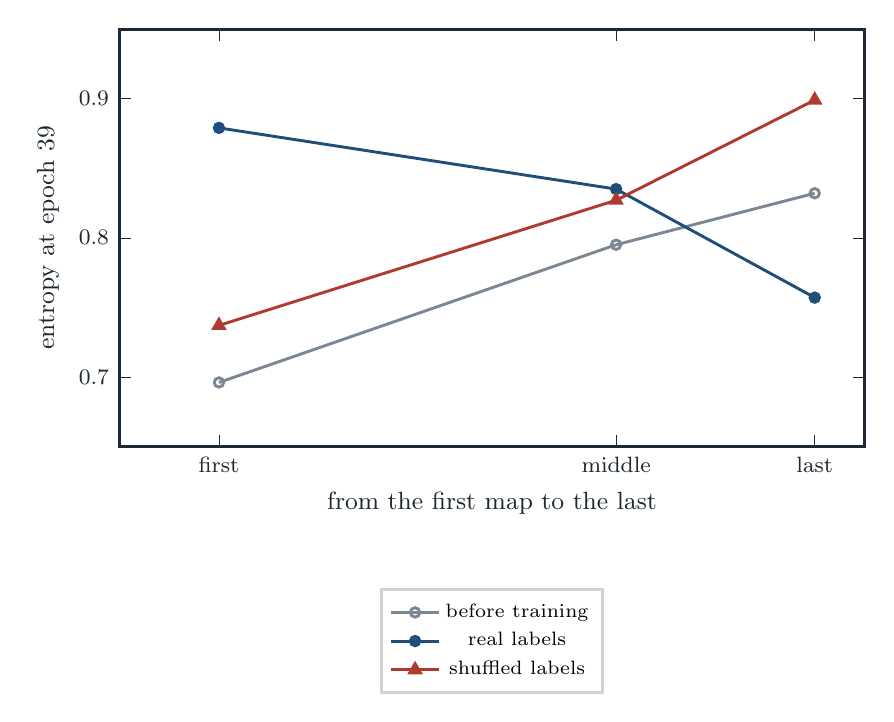
\begin{tikzpicture}
\begin{axis}[
  xlabel={from the first map to the last},
  ylabel={entropy at epoch 39},
  xmin=6, xmax=36,
  ymin=0.65, ymax=0.95,
  xtick={32,16,8},
  xticklabels={first, middle, last},
  x dir=reverse,
  width=0.78\linewidth,
  height=5.3cm,
  legend style={at={(0.5,-0.34)}, anchor=north, legend columns=1, font=\scriptsize},
]
\addplot[muted, mark=o, mark size=1.7pt] coordinates {(32,0.696) (16,0.795) (8,0.832)};
\addlegendentry{before training}
\addplot[real, mark=*, mark size=1.7pt] coordinates {(32,0.879) (16,0.835) (8,0.757)};
\addlegendentry{real labels}
\addplot[rand, mark=triangle*, mark size=2.2pt] coordinates {(32,0.737) (16,0.827) (8,0.899)};
\addlegendentry{shuffled labels}
\end{axis}
\end{tikzpicture}
\caption{All three maps at the end.}
\label{fig:profile}
\end{subfigure}
\caption{The first map is the one nearest the picture. The last map is the \(8\times 8\) map from Figure~\ref{fig:entropy}.}
\label{fig:depth}
\end{figure}

The split is not the same at every depth.
With real labels, the first map becomes more spread out, from \(0.70\) to \(0.88\), while the last map becomes more concentrated, from \(0.83\) to \(0.76\).
With shuffled labels, the first map barely moves, and the last map is the one that spreads, ending at \(0.90\).
The middle map stays between them.

The same parting of the lines shows up beyond this one comparison. On the full set of \(50{,}000\) pictures the real-label entropy ends at \(0.76\), with test accuracy \(0.90\). The shuffled-label entropy ends at \(0.88\), with test accuracy \(0.09\), and again the entropy is already above its starting value while training accuracy on the shuffle is still \(0.16\).

Changing the random starting weights, among the standard choices, leaves the real-label result in place: entropy ends between \(0.75\) and \(0.79\). Flipping \(20\%\) or \(40\%\) of the labels, while keeping cropping and the weight penalty, also stays on that side. Entropy ends at \(0.77\) in both cases, and test accuracy is still \(0.74\) and \(0.67\). A mild amount of wrong labels is not the same thing as a fully shuffled target.

\begin{table}[ht]
\centering
\caption{Where each setting finishes.
Entropy is the last map, on real test pictures.
Training accuracy uses the labels the run was given.
Test accuracy uses the true labels.}
\label{tab:endpoints}
\small
\begin{tabular}{@{}lrrrr@{}}
\toprule
Setting & Train & Test & Entropy at start & Entropy at end \\
\midrule
Real labels, with augmentation & 0.95 & 0.81 & 0.83 & 0.76 \\
Real labels, no augmentation & 1.00 & 0.77 & 0.83 & 0.79 \\
Shuffled labels, with augmentation & 0.14 & 0.10 & 0.83 & 0.79 \\
Shuffled labels, no augmentation & 0.48 & 0.10 & 0.83 & 0.90 \\
\midrule
Full set, real labels & 0.98 & 0.90 & 0.83 & 0.76 \\
Full set, shuffled labels & 0.16 & 0.09 & 0.83 & 0.88 \\
\midrule
20\% of labels flipped & 0.69 & 0.74 & 0.83 & 0.77 \\
40\% of labels flipped & 0.49 & 0.67 & 0.83 & 0.77 \\
\bottomrule
\end{tabular}
\end{table}

Read together, the graphs say something narrow. When the labels still carry the real categories, the last map becomes more concentrated and stays that way, including the case where the training set is memorized exactly. When the labels are a pure shuffle and nothing discourages fitting them, the last map becomes more spread out, and this shows up on ordinary test pictures before the fit to the shuffle is obvious in the accuracy.

\section{Methodology}

Every curve above comes from the same small image network, trained on CIFAR-10. The network has three stages and about \(1.15\) million parameters. Each stage is two small convolutions, with a normalization step and a unit that keeps only positive values. A pooling step sits between stages. On a \(32\times 32\) picture the three hidden maps are \(32\times 32\), \(16\times 16\), and \(8\times 8\). Entropy is computed on each of them. The last map is the one in Figure~\ref{fig:entropy}. A still smaller map would have too few frequencies for the number to mean much.

\begin{figure}[H]
\centering
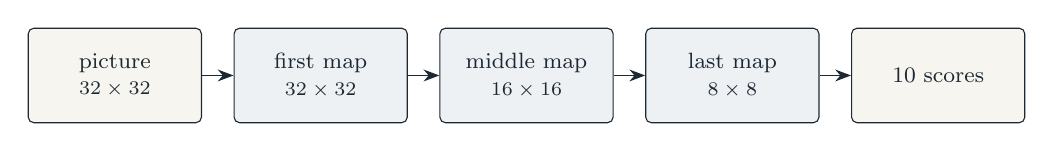
\begin{tikzpicture}[
  font=\footnotesize,
  stage/.style={draw=ink, rounded corners=2pt, align=center, inner sep=4pt, fill=paper, text=ink, minimum width=22mm, minimum height=12mm},
  arr/.style={-{Stealth[length=2mm]}, semithick, ink}
]
  \node[stage] (in) {picture\\{\scriptsize $32\times 32$}};
  \node[stage, right=4mm of in, fill=real!8] (b32) {first map\\{\scriptsize $32\times 32$}};
  \node[stage, right=4mm of b32, fill=real!8] (b16) {middle map\\{\scriptsize $16\times 16$}};
  \node[stage, right=4mm of b16, fill=real!8] (b8) {last map\\{\scriptsize $8\times 8$}};
  \node[stage, right=4mm of b8] (y) {10 scores};
  \draw[arr] (in) -- (b32);
  \draw[arr] (b32) -- (b16);
  \draw[arr] (b16) -- (b8);
  \draw[arr] (b8) -- (y);
\end{tikzpicture}
\caption{The network behind the graphs. Entropy is measured on the three shaded maps.}
\label{fig:net}
\end{figure}

The matched comparison uses one fixed subset of \(10{,}000\) training pictures, shared by every run. A second pair uses all \(50{,}000\). Training is ordinary gradient descent with momentum, batch size \(256\), and a learning rate that starts at \(0.1\) and falls smoothly to zero. Where augmentation is on, each picture is randomly cropped and sometimes flipped, and large weights are penalized. Where it is off, neither of those is used.

The shuffle is drawn once. Repeating a run changes the starting weights and the order of the batches. It does not change which picture carries which shuffled label. Entropy is always measured on the real test pictures, with the network in its evaluation setting, and it is not part of the training loss. Training accuracy is scored on the labels the run actually received. Test accuracy is scored on the true labels.

\begin{center}
\small
\begin{tabular}{@{}llc@{}}
\toprule
Line on the graphs & Labels & Augmentation and weight penalty \\
\midrule
Blue, solid & real & on \\
Green, dashed & real & off \\
Grey, dashed & one fixed shuffle & on \\
Red, solid & one fixed shuffle & off \\
\bottomrule
\end{tabular}
\end{center}

Two further settings use real labels with augmentation left on. One tries three other standard ways of choosing the starting weights. The other flips \(20\%\) or \(40\%\) of the training labels to a different class. The full-set runs repeat only the blue and red settings.

\section{Earlier uses of the same formula}

The same entropy, with a different choice of what counts as a frequency, was measured on other models before the graphs above. Those numbers are not entropies of a hidden picture. They are included so the two uses of the formula are not mixed up.

For pretrained image networks, the energy at each scale was the average squared weight of a layer, and the scale was the size of the region that layer can see. Entropy is then an entropy over layers. It is \(0.57\) of its maximum for AlexNet, and about \(0.28\) for VGG-16 and VGG-19, because the first layer holds most of the average weight energy. Using the total squared weight instead, which grows in later layers simply because they have more weights, pushes the same ratio up to about \(0.95\). The choice of average versus total changes the conclusion, which is one reason the graphs in this note normalize the frequency energies and report a number between 0 and 1.

On a pretrained residual network the activation energy is nearly flat across stages, while the weight energy still declines toward finer scales. During training of a plain fully connected network, the activation energies become more evenly spread and the weight energies become less so.

For GraphCast, energy at a mesh level comes from the encoder acting on edge geometry alone, with no weather fed in. That entropy is \(1.21\) bits on all three public checkpoints, about \(43\%\) to \(47\%\) of the maximum, and most of the energy sits on the coarsest mesh. The learned activations on a real forecast are much flatter: mean energy per edge falls only gently toward fine scales, and the variation around that mean stays spread out. Forecast fields themselves, such as temperature, pressure, and wind, fall off much more steeply with scale.

For FourCastNet the check so far is a control. On noise with no atmospheric structure, energy binned by frequency ring grows in the way geometry requires, and the entropy barely moves from the first block to the last. A real weather input has not been run through that measurement yet.

\end{document}
